\section{NAO - The Humanoid Robot} NAO is an autonomous programmable humanoid robot invented by Aldebaran Robotics. NAO Academics Edition is developed for universities and laboratories for research and educational purposes. Follow subsections discuss briefly about the specifications of NAO as described by Aldebaran Robotics \cite{8}.

\begin{table}
	[h] \centering \caption{NAO V5 specification } \label{tb:nao:spec} 
	\begin{tabular}
		{|l|l|} \hline Height & 58 centimetres (23 in) \\
		\hline Weight & 4.3 kilograms (9.5 lb) \\
		\hline Battery autonomy & 60 minutes (active use), 90 minutes (normal use) \\
		\hline Degrees of freedom & 21 to 25 \\
		\hline CPU & Intel Atom @ 1.6 GHz \\
		\hline Built-in OS & Linux \\
		\hline SDK compatibility & Windows, Mac OS, Linux \\
		\hline Programming languages & C++, Python, Java, MATLAB, Urbi, C, .Net \\
		\hline Vision & 2 x HD 1280x960 cameras \\
		\hline Connectivity & Ethernet, Wi-Fi \\
		\hline \multirow{6}{*}{Sensors} & 4 x directional microphones \\
		& 1 x sonar rangefinder \\
		& 2 x IR emitters and receivers \\
		& 1 x inertial board \\
		& 9 x tactile sensors \\
		& 8 x pressure sensors \\
		\hline 
	\end{tabular}
\end{table}


\subsection{Body} NAO has a body with 25 degrees of freedom (DOF) whose key elements are electric motors and actuators as show in the figure \ref{fg:nao:body}. It has 48.6-watt-hour battery that provides 1.5 or more hours of autonomy, depending on the usage. Additional specifications of robot are shown in the table \ref{tb:nao:spec}. 

\begin{figure}
	\begin{minipage}
		{.6
			\textwidth} 
		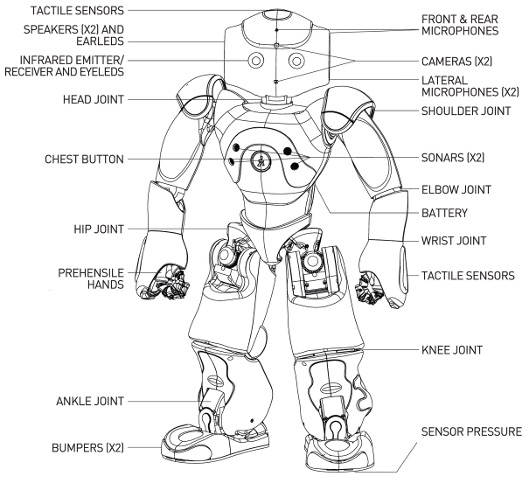
\includegraphics[height=7cm]{figures/content/nao-body.jpg} 
	\end{minipage}
	\begin{minipage}
		{.4 
			\textwidth} 
		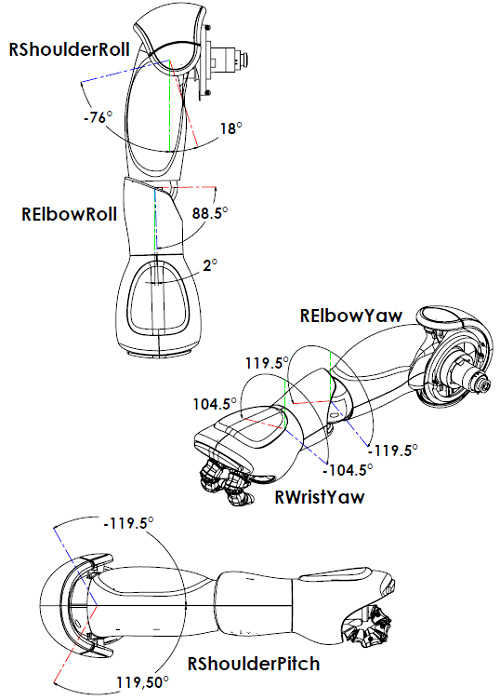
\includegraphics[height=7cm]{figures/content/nao-hand.jpg} 
	\end{minipage}
	\begin{minipage}
		{.6 
			\textwidth} 
		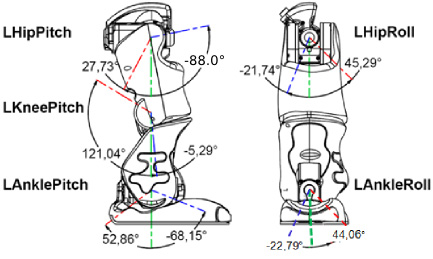
\includegraphics[height=50mm]{figures/content/nao-leg.jpg} 
	\end{minipage}
	\begin{minipage}
		{.4 
			\textwidth} 
		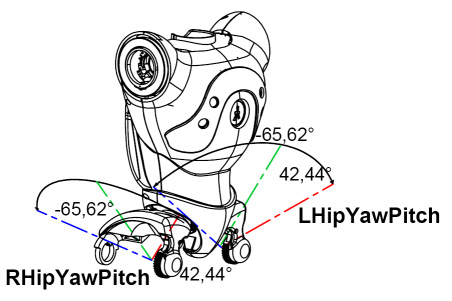
\includegraphics[height=40mm]{figures/content/nao-hip.jpg} 
	\end{minipage}
	\caption{Shoulder, Leg and Hip joints illustrating the body construction of NAO V5 \cite{nao-spec}} \label{fg:nao:body} 
\end{figure}


\subsection{Motion} NAOs walking algorithm uses a simple dynamic model (linear inverse pendulum) and quadratic programming. It is stabilized using feedback from the joint sensors. This makes the walking robust and resistant to small disturbances, and torso oscillations in the frontal and lateral planes are absorbed. It can walk on a variety of floor surfaces, such as carpeted, tiled, and wooden floors. 

NAOs motion module is based on generalized inverse kinematics, which handles locomotion, joint control, balance, redundancy, and task priority. This means that when asking it to extend its arm, it bends over because its arms and leg joints are taken into account.

\begin{figure}
	\centering 
	\begin{minipage}
		{.3 
		\textwidth} \centering 
		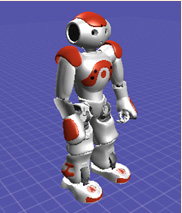
\includegraphics[height=5cm]{/content/nao-stand.jpg} 
	\end{minipage}
	\begin{minipage}
		{.3 
		\textwidth} \centering 
		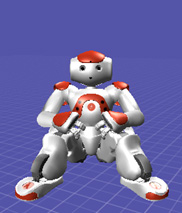
\includegraphics[height=5cm]{/content/nao-sit.jpg} 
	\end{minipage}
	\begin{minipage}
		{.3 
		\textwidth} \centering 
		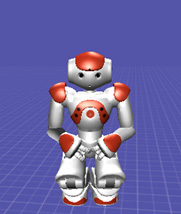
\includegraphics[height=5cm]{/content/nao-crouch.jpg} 
	\end{minipage}
	\caption{Standing, Sitting and Crouching postures of virtual NAO using ALRobotPosture module. \cite{8}} \label{fg:nao:motion} 
\end{figure}


In this thesis, we attempt to use the locomotion and stiffness control of Motion API to move NAO to a position in the two dimensional space. Robot Posture API will also be used to make the robot go to the predefined posture such as Stand, Sit and Crouch as shown in the figure \ref{fg:nao:motion}.

\subsection{Audio} NAO uses four directional microphones to detect sounds and equipped with a stereo broadcast system made up of 2 loudspeakers in its ears as shown in the figure \ref{fg:nao:audio}. NAOs voice recognition and text-to-speech capabilities allow it to communicate in 19 languages. 

\begin{figure}
	[h] \centering 
	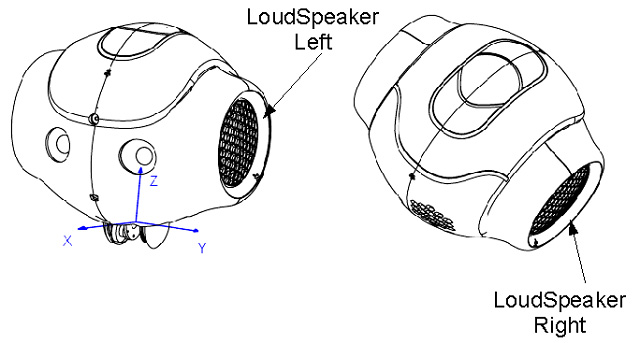
\includegraphics[height=7cm]{figures/content/nao-audio.jpg} \caption{NAO Audio} \label{fg:nao:audio} 
\end{figure}
 

In this thesis, we aim to use Text-To-Speech API of NAO to say the detected gesture loud to communicate with the user.

\begin{figure}
	[h] \centering 
	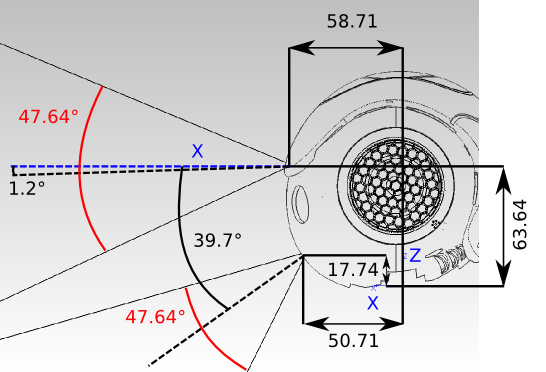
\includegraphics[height=7cm]{figures/content/nao-vision.jpg} \caption{The field of view of two identical RGB video cameras which are located in the forehead of NAO. \cite{8} } \label{fg:nao:vision} 
\end{figure}


\subsection{Vision} \label{sec:nao:vision} Proper vision is the utmost importance for the function of any vision based autonomous robot. Areas of artificial intelligence deal with autonomous planning or deliberation for robotic systems to navigate through an environment. High-level information about the environment could be provided by a computer vision system that is acting as a vision of the robot.

Two identical video RGB cameras are located in the forehead of NAO as shown in the figure \ref{fg:nao:vision}. They provide up to 1280x960 resolution at 30 frames per second. Aldebaran provides a set of algorithms for detecting and recognizing faces and shapes.

\paragraph*{Depth Image} Skeletal points based gesture recognition needs three dimensional data of the human skeleton. However, sensors integrated with NAO could not provide precise three dimensional data to the sophisticated algorithms to track human skeletal joints \cite{17}. 3D cameras such as Microsoft Kinect and Asus Xtion are used not only for gaming but also for analyzing 3D data, including algorithms for feature selection, scene analysis, motion tracking, skeletal tracking and gesture recognition \cite{9} \cite{18}. Therefore, we seek to utilize Asus Xtion PRO LIVE as an external camera to support the skeletal points tracking system of NAO. 

\begin{figure}
	[h] \centering 
	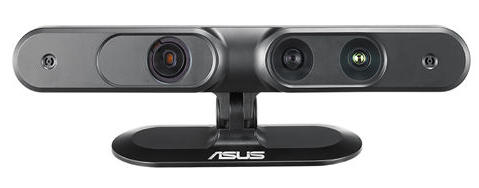
\includegraphics[height=4cm]{figures/content/xtion.png} 
	\caption{Asus Xtion Pro Live}
	\label{fg:xtion} 
\end{figure}

\paragraph*{Asus Xtion} Figure \ref{fg:xtion} shows Asus Xtion PRO LIVE that uses infrared sensors, adaptive depth detection technology, color image sensing and audio stream to capture a 3D image of the user in real-time. It uses infrared emitters to project speckle patterns on the object and uses a structured light technique to compute the depth of the image. Once the depth image is computed, it is mapped onto the RGB image as shown in the figure \ref{fg:xtion:depth}. Lighter color denote that a pixel is closer to the camera and darker color denotes that a pixel is far from the camera.

\begin{figure}
	[h] \centering 
	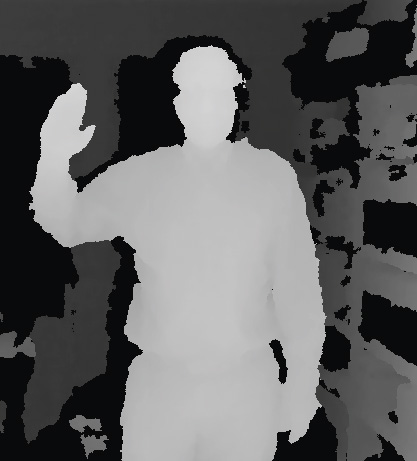
\includegraphics[height=8cm]{figures/content/xtion-depth.jpg} 	
	\caption{Depth Image recorded by depth camera Asus Xtion Pro Live} \label{fg:xtion:depth} 
\end{figure}


\subsection{Computing} NAO is equipped with Intel ATOM 1.6 GHz CPU in the head that runs a 32 bit Gentoo Linux to support Aldebarans proprietary middleware (NAOqi). NAOqi SDK is the programming framework used to program Aldebaran robots \cite{8}. This framework allows homogeneous communication between different modules such as motion, audio and video. NAOqi executable that runs on the robot is a broker. The broker provides lookup services so that any module in the tree or across the network can find any method that has been advertised as shown in the figure \ref{fg:nao:proxy}.

\begin{figure}
	[h] \centering 
	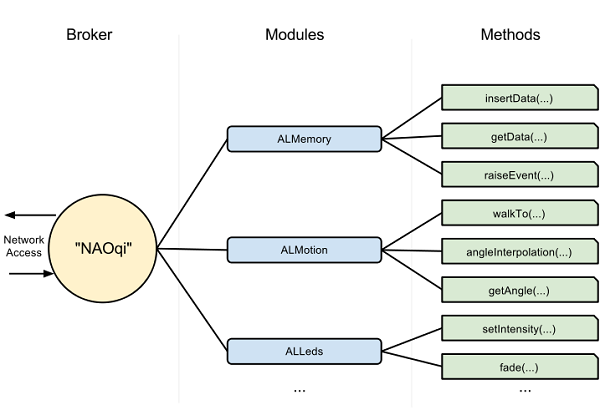
\includegraphics[height=7cm]{figures/content/nao-proxy.png} 
	\caption{NAOqi Proxy}
	\label{fg:nao:proxy} 
\end{figure}

Computational limitations \cite{17} of NAO CPU hinders us to build a real time gesture recognition based on human skeletal joints. Thus, we aim to use an off-board computer to execute the gesture recognition program and communicated with NAO via NAOqi proxies. 
